\section{Lucene}

Dans cette première partie, nous abordons Lucene, le moteur de recherche que nous avons choisi d’évaluer. Après une présentation général du projet Lucene, nous donnons un aperçu de son fonctionnement pour ensuite entrer dans les détails des composants pouvant être configurées.

\subsection{Généralités}

Lucene est une bibliothèque libre codée en Java proposant des fonctionnalités avancées d’indexation et de recherche de documents. Elle a été créée en 1999 par Doug Cutting, qui a par ailleurs créé Hadoop, très utilisé dans le domaine de la Big Data. Lucene devient en 2001 un projet Apache, lui conférant ainsi une certaine notoriété auprès du public.

Avant l’explosion d’Internet, la masse et la variété des documents présents sur la Toile étaient encore modestes : la méthode de recherche plébiscitée était la classification décimale de Dewey, dont s’inspire encore les bibliothèques. Avec cette méthode, il y a 3 niveaux de classification : les classes, les divisions et les sections. Les classes sont au nombre de 10. On retrouve par exemple la classe “religion”, la classe “langues”, la classe “sciences sociales”, etc. Les divisions sont l’équivalent des sous-catégories, elles sont au nombre de 100. Enfin, les sections permettent une nouvelle fois de raffiner la catégorie des documents classés, elles sont au nombre de 1000.

Bien que cette classification soit intuitive, elle pose de multiples problèmes : elle est assez statique et doit être modifiée quand de nouveaux types de documents apparaissent, elle ne permet pas les recherches ciblées sur des mots-clés et les recherches ne sont pas efficaces dû au trop grand nombre d’indirections. Enfin, l’explosion du nombre de documents disponibles sur Internet a montré les limites de cette classification : même avec 1000 sections différentes, le nombre de documents disponibles dans chacune des catégories est devenu trop important.

Pour explorer le web, la méthode de référence est devenue la recherche par mots-clés, elle est aujourd’hui utilisée par la très grande majorité des moteurs de recherche grand public. Pour permettre une recherche rapide et efficace parmi la masse importante de documents, une nouvelle approche était nécessaire : c’est celle que fournit Lucene.

La bibliothèque est aujourd’hui utilisée par des sites web comme Wikipedia, Akamai ou SourceForge ; mais elle est aussi utilisée par des applications telles que Eclipse, JIRA, Nutch ou Solr (ces deux dernières applications étant elles-mêmes des outils de plus haut niveau que Lucene facilitant la mise en place d’un moteur de recherche). Grâce à ses très bonnes performances et sa fiabilité, elle est au cœur de nombreux projets traitant de la récupération d’informations.

\subsection{Fonctionnement général}

Pour s’affranchir de potentiels problèmes de format (PDF, HTML, Word, etc.), Lucene a créé sa propre abstraction. Ainsi, l’objet manipulé par la bibliothèque logicielle est le document, qui est composé d’un ou plusieurs champs qui contiennent du texte.
L’utilisation de Lucene est décomposée en deux grandes parties : la première étape consiste en l’indexation des documents. C’est seulement après cette étape que l’on pourra interroger Lucene pour retrouver les documents correspondants à une requête de l’utilisateur.

\subsubsection{Indexation}

Pour cette première étape, il faut avant tout extraire le texte que l’on veut indexer d’un fichier HTML, PDF ou Word (cette tâche n’est pas assurée par Lucene et est à la charge du programmeur). Ensuite, il faut en créer un document. Par exemple, si l’on veut indexer une bibliothèque pour permettre à ses usagers de trouver un livre à partir de mots-clés de son résumé, on pourra utiliser la modélisation suivante pour les documents :

Le document représente un livre :
\begin{itemize}
  \item Un champ ISBN pour identifier un livre de manière unique
  \item Un champ titre
  \item Un champ auteur
  \item Un champ résumé
  \item Un champ rayon pour permettre de retrouver le livre dans la bibliothèque
\end{itemize}

~~\\
On remarque que tous les champs ne seront pas utiles à la recherche. Par exemple, l’usager d’une bibliothèque ne recherchera jamais un livre suivant sa position en rayon : s’il sait déjà où se trouve le livre, il saura déjà quel est le titre du livre, qui en est l’auteur, etc. En revanche, si l’utilisateur recherche un livre à partir de mots-clés du résumé, il peut être intéressant de lui indiquer où il se trouve dans la bibliothèque. Ainsi, le champ d’un document Lucene dispose de deux paramètres de configuration : “indexed” qui indique à Lucene via une valeur booléenne si le champ pourra faire l’objet d’une requête de l’usager (le paramètre sera par exemple à vrai pour le champ résumé, mais à faux pour le champ rayon), et “stored” qui indique si le champ sera affiché dans les résultats de la recherche. La performance de la recherche dépendra de ces paramètres. De manière logique, si l’on rend tous les champs cherchables (“indexed” à vrai), la recherche sera plus longue.

Une fois que le problème est modélisé sous forme de documents et de champs, et que ces derniers sont correctement configurés, nous pouvons procéder à l’indexation. Un index n’est rien d’autre qu’une forme condensée des documents en entrée permettant une recherche rapide et efficace. L’indexation permettra de créer et de mettre à jour l’index, tandis que l’interrogation se contentera de le consulter pour répondre à une requête de l’utilisateur.

\subsubsection{Interrogation}

L’étape d’interrogation peut devenir très complexe si l’on veut utiliser toutes les possibilités de recherche de Lucene, mais nous nous contentons dans cette partie de la version la plus basique.

Dans un premier temps, l’utilisateur entre sa requête : sur quel(s) terme(s) veut-il effectuer sa recherche ? Il revient ensuite au programmeur de faire l’intermédiaire entre l’utilisateur et Lucene : il faut configurer la recherche, en indiquant les champs dans lesquels on veut chercher les termes entrés par l’utilisateur (leurs paramètres de configuration “indexed” doivent obligatoirement être vrais), et les champs que l’on veut récupérer dans les résultats de la recherche (leurs paramètres de configuration “stored” doivent obligatoirement être vrais). Après consultation de l’index, Lucene nous renvoie des résultats et associe à chaque réponse un score, qui estime la pertinence du document retourné au vue de la requête de l’utilisateur.

Lucene propose de nombreuses autres possibilités de recherche : possibilité de trier les résultats sur un champ, possibilité de filtrer les résultats en fonction de la valeur d’un champ, possibilité de mise en surbrillance des termes d’un champ répondant à la requête de l’utilisateur, etc. Ces différentes fonctionnalités ne seront pas utiles à notre étude, et ne seront donc pas détaillées.

\subsubsection{Synthèse}

Une illustration synthétisant les concepts évoqués précédemment est disponible en annexe //TODO//, elle permet de distinguer clairement les responsabilités des différents acteurs (l’utilisateur, le programmeur et la bibliothèque logicielle Lucene) et indique le déroulement de l’indexation (à gauche) et de l'interrogation (à droite).

 \begin{figure}[h]
            \centering
            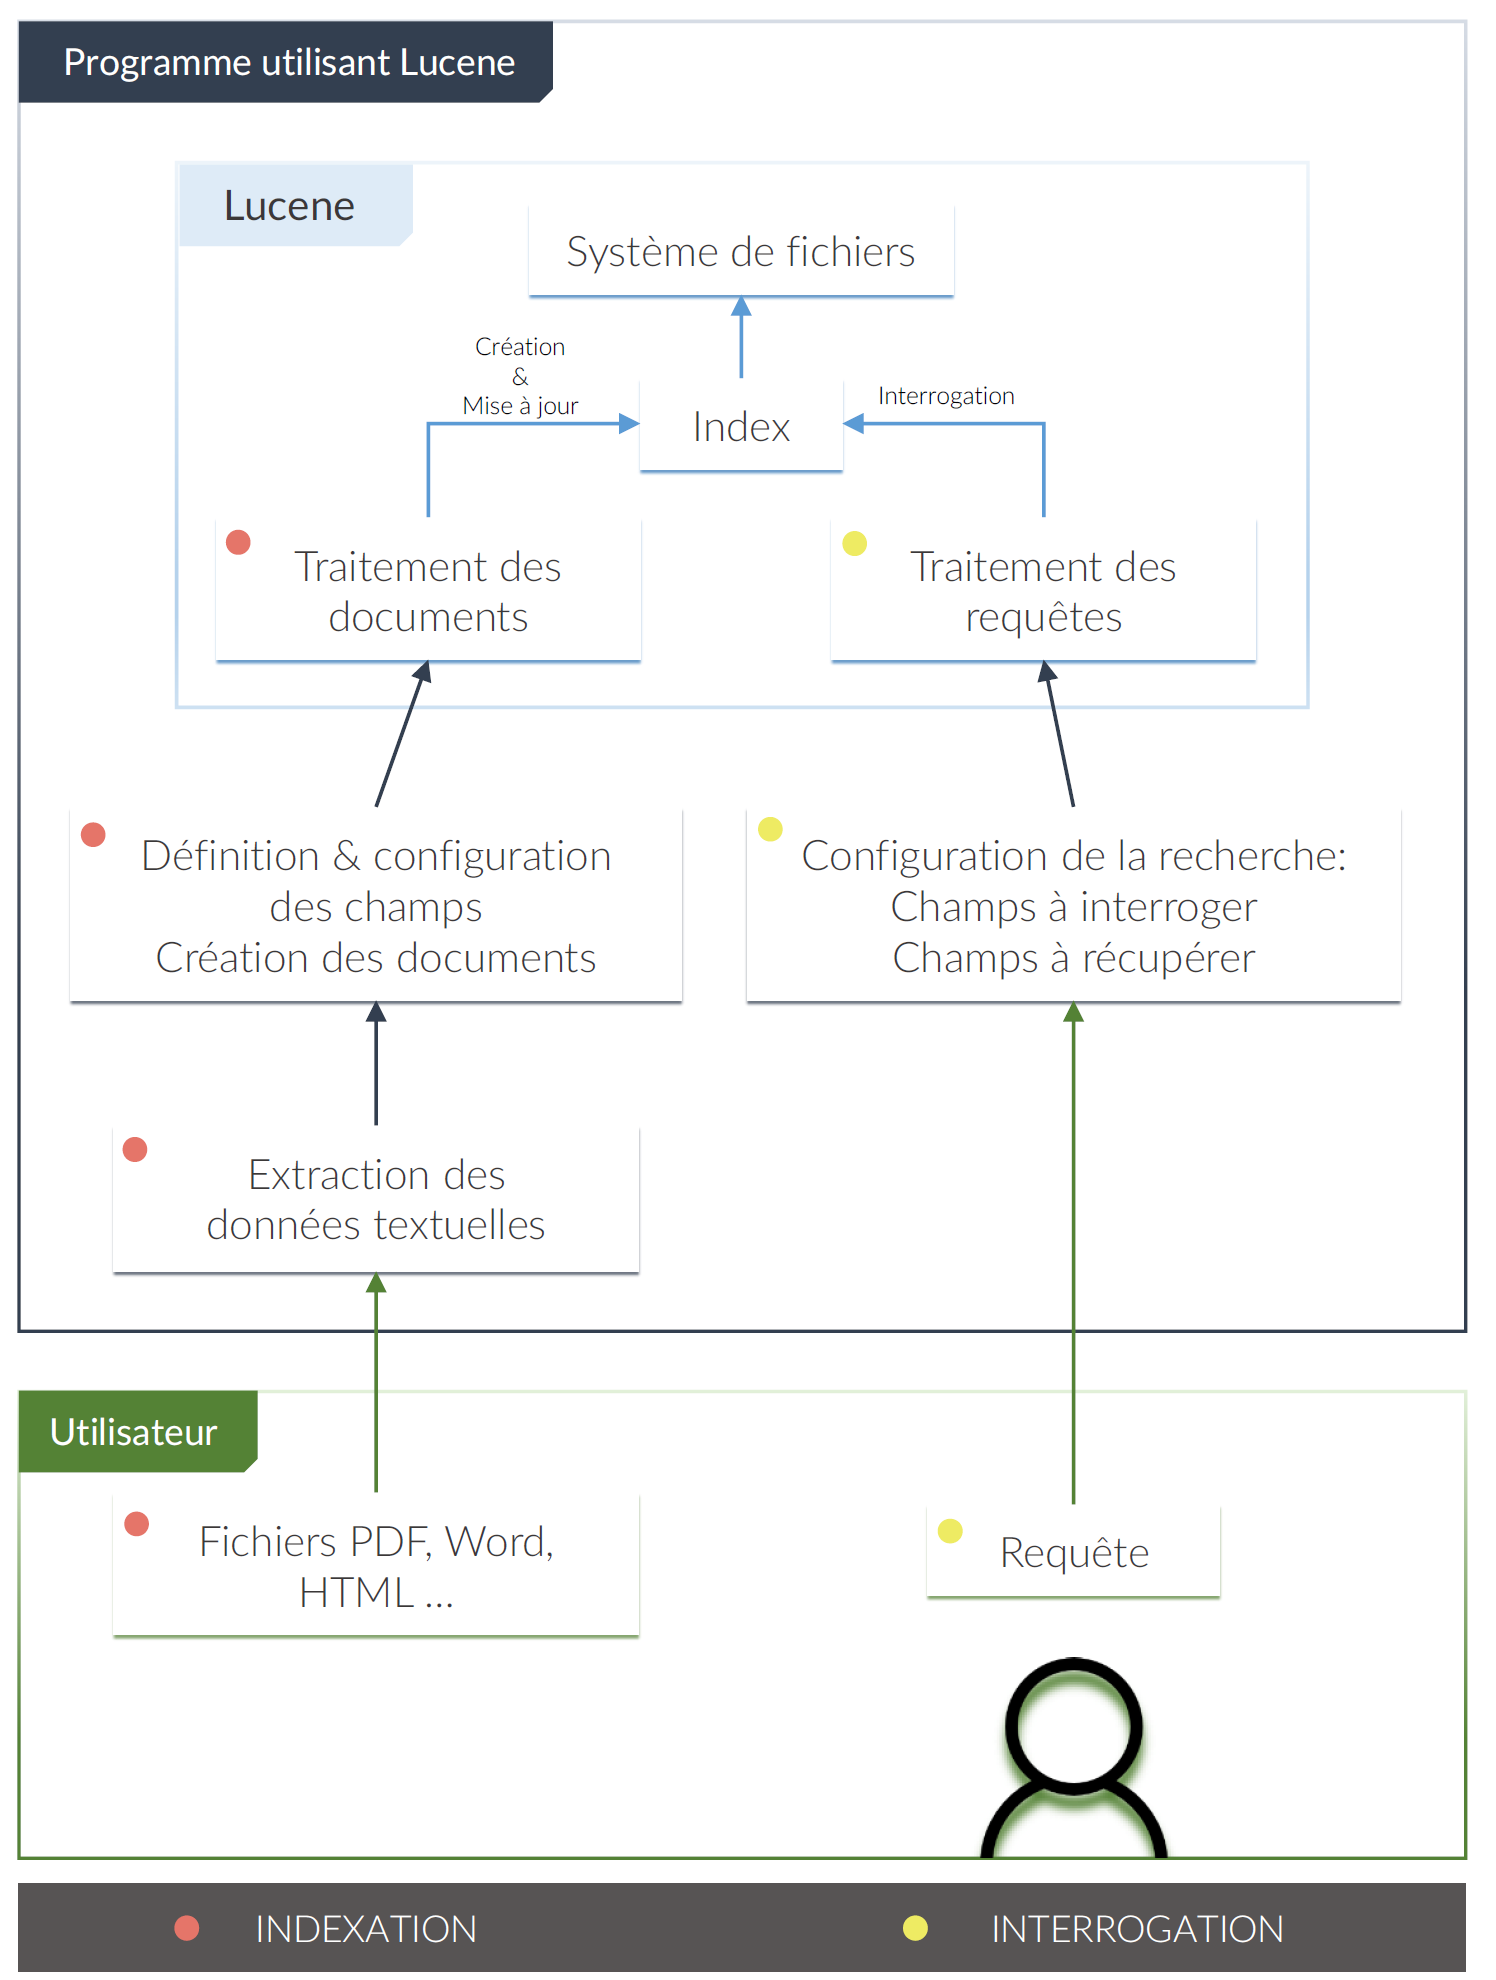
\includegraphics[width=1\textwidth]{figure/fonctionnement.jpg}
            \caption{Fonctionnement programme}
            \label{fig:fonctionnement_prog}
 \end{figure}

\subsection{Analyseur}

Pour permettre une recherche efficace, le texte contenu dans les champs d’un document est transformé en une succession de termes. Cette étape est fondamentale pour assurer la pertinence des résultats : cela permettra par exemple de trouver une correspondance entre un verbe conjugué dans un document et un verbe à l’infinitif dans la requête d’un utilisateur. Il s’agira dans un premier temps de pouvoir distinguer les différents termes de la phrase, grâce au découpage en termes (tokenization en anglais). C’est sur ces termes qu’on appliquera des transformations, grâce au filtrage.

\subsubsection{Le découpage en termes}

Lucene met à disposition plusieurs tokenizers prédéfinis, dont le fonctionnement est synthétisé dans le tableau //TODO//. Pour illustrer leurs actions, la troisième colonne donne les différents termes produits pour le texte d’entrée “Voit-on J.M. demain ?”.
 
            \begin{table}[H]
                \centering
                \begin{tabular}{|p{4.5cm}|p{4.5cm}|p{4.5cm}|}
                    \hline
                    \textbf{Nom} & \textbf{Fonctionnement} & \textbf{Termes produits}\\
                    \hline
                    KeywordTokenizer & Transforme l’ensemble du texte d’entrée en un unique terme & “Voit-on J.M. demain ?”\\
		\hline
                    WhitespaceTokenizer & Crée un nouveau terme à chaque espace blanc & “Voit-on” “J.M.” “demain”\\
		\hline
                    StandardTokenizer & Crée un nouveau terme à chaque séparateurs de mots couramment rencontrés dans les langages & “Voit” “on” “J.M.” “demain”\\
		\hline
                    LetterTokenizer & Crée un nouveau terme à chaque séparation de mots & “Voit” “on” “J” “M” “demain”\\
		\hline
                    LowerCaseTokenizer & Crée un nouveau terme à chaque séparation de mots en enlevant les majuscules & “voit” “on” “j” “m” “demain”\\
                    \hline

                \end{tabular}
                \caption{Découpage des termes}
                \label{tab:decoupage_termes}
            \end{table}

\subsubsection{Le filtrage des termes}

Après le découpage en termes vient l’étape de filtrage, pendant laquelle chacun des termes va être passé en revue. Ce traitement permettra soit de supprimer, soit de modifier, soit de créer de nouveaux termes. Le tableau //TODO// donne un aperçu des filtres les plus courants, et montre leurs effets sur des exemples :

\begin{table}[H]
                \centering
                \begin{tabular}{|p{3cm}|p{3cm}|p{3cm}|p{3cm}|}
                    \hline
                    \textbf{Nom} & \textbf{Fonctionnement} & \textbf{Termes en entrée} & \textbf{Termes produits}\\
                    \hline
LowerCaseFilter & Transforme le terme en lettres minuscules & “France” & “france”\\
\hline
ApostropheFilter & Supprime tous les caractère suivant une apostrophe, et l’apostrophe elle-même & “aujourd’hui” & “aujourd”\\
\hline
ClassicFilter & Supprime les points des acronymes et les “‘s” finaux & "I.B.M. cat's can't" & “IBM” “cat” “can’t”\\
\hline
StopFilter & Supprime les termes les plus courants d’un langage n’ayant pas de signification particulière (mots vides) & “match” “de” “foot” & “match” “foot”\\
\hline
EdgeNGramFilter & Crée des sous-préfixes de chaque mot & “Apache” & “Ap”, “Apa”, “Apac”, “Apach”, “Apache”\\
\hline
ASCIIFoldingFilter & Transforme les caractères accentués en leurs équivalents non accentués & “équipe” & “equipe”\\
\hline
SynonymFilter & Produit les synonymes d’un terme & “patate” & “pomme de terre”, “patate”\\
\hline
WordDelimiterFilter & Concatène/découpe des termes en fonction des particularités des langages & “Wi-Fi” “PowerShot” & “WiFi” “Wi” “Fi” “Power” “Shot”\\
\hline
SnowballFilter & Réduit les termes à leurs formes radicalisées (ou une forme qui s’en approche) & “cheval”  “chevaux”  “peigne” & “cheva" “cheva” "peign”\\
                    \hline

                \end{tabular}
                \caption{Filtrage des termes}
                \label{tab:filtrage_termes}
            \end{table}

Il existe bien d’autres filtres, et ceux détaillés dans le tableau ont parfois de nombreux paramètres de configuration. Par exemple, on peut fournir au filtre StopFilter sa propre liste de mots vides. De manière similaire, on peut fournir sa propre liste de synonymes au filtre SynonymFilter. Le filtre SnowballFilter peut quant à lui être configuré pour traiter du texte dans un certain langage, afin d’optimiser les résultats.

\subsubsection{Utilité de l'analyseur}

Nous avons initialement décrit l’analyse (découpage et filtrage des termes) comme un traitement ayant lieu lors de la phase d’indexation. En réalité, l’analyseur est aussi utilisé lors de la phase d’interrogation et permet de transformer la requête de l’utilisateur pour trouver des correspondances dans l’index. Pour comprendre l’utilité de l’analyseur, nous détaillons des résultats de recherche suivant différentes configurations de l’analyseur dans le tableau //TODO//. L’analyse poussée évoquée dans la première colonne décrit l’utilisation d’un StandardTokenizer avec les filtres suivants : LowerCaseFilter, StopFilter, ISOLatin1AccentFilter et SnowballFilter.

\begin{table}[H]
                \centering
                \begin{tabular}{|p{2.3cm}|p{2.3cm}|p{2.3cm}|p{2.3cm}|p{2.3cm}|p{2.3cm}|}
                    \hline
                    \textbf{Configuration de l’analyseur} & \textbf{Texte en entrée} & \textbf{Texte analysé} & \textbf{Correspondance} & \textbf{Requête analysée} & \textbf{Requête en entrée}\\
                    \hline                    
Analyse minimale en indexation et en interrogation (seulement un découpage en termes) & Je pense que nous disposons d’assez de preuves pour dire que Lucene est plutôt utile ! & Je, pense, que, nous, disposons, d’assez, de, preuves, pour, dire, que, Lucene, est, plutôt, utile & //TO DO// & preuve, utilité, lucene & preuve utilité lucene\\
		\hline
Analyse poussée seulement en indexation & Je pense que nous disposons d’assez de preuves pour dire que Lucene est plutôt utile ! & je, pens, nous, dispos, assez, preuv, dir, lucene, util & OK lucene & preuve, utilité, lucene & preuve utilité lucene\\
		\hline
Analyse poussée en indexation et en interrogation & Je pense que nous disposons d’assez de preuves pour dire que Lucene est plutôt utile ! & je, pens, nous, dispos, assez, preuv, dir, lucene, util & OK preuv lucene util & preuv, util, lucene & preuve utilité lucene\\
                    \hline

                \end{tabular}
                \caption{Utilité Analyseur}
                \label{tab:utilité_analyseur}
            \end{table}

On remarque immédiatement l’intérêt des analyseurs, en indexation comme en interrogation. Dans le dernier cas de figure, on a en effet trouvé un nombre important de correspondances entre la requête de l’utilisateur et le document indexé. Ce nombre de correspondances est très important, il détermine en effet le score du document dans les résultats, qui est le seul moyen mis à disposition par Lucene pour trier les résultats par pertinence. C’est donc ce qui fera la qualité des résultats renvoyés lors de la recherche dans des millions de documents.





